% The half-disc, rectangle and square contours, with the poles they enclose. Generated by a short script.
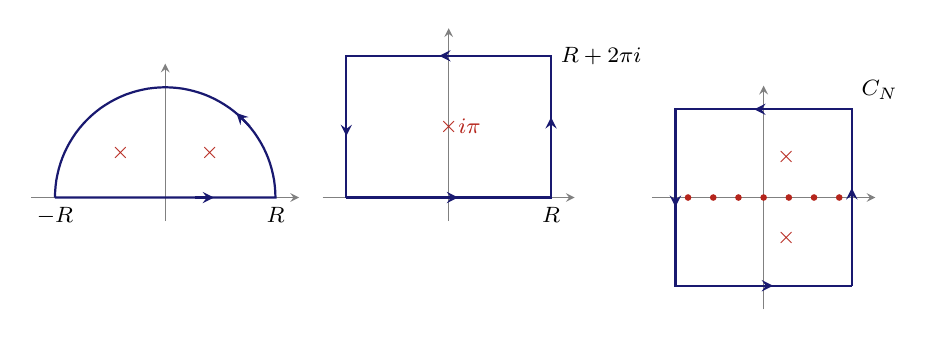
\begin{tikzpicture}[every node/.style={font=\footnotesize},>=stealth]
\draw[->,gray] (-1.70,0)--(1.70,0);\draw[->,gray] (0,-0.3)--(0,1.70);
\draw[MidnightBlue,thick] (-1.400,0.000)--(1.400,0.000)--(1.398,0.073)--(1.392,0.146)--(1.383,0.219)--(1.369,0.291)--(1.352,0.362)--(1.331,0.433)--(1.307,0.502)--(1.279,0.569)--(1.247,0.636)--(1.212,0.700)--(1.174,0.762)--(1.133,0.823)--(1.088,0.881)--(1.040,0.937)--(0.990,0.990)--(0.937,1.040)--(0.881,1.088)--(0.823,1.133)--(0.762,1.174)--(0.700,1.212)--(0.636,1.247)--(0.569,1.279)--(0.502,1.307)--(0.433,1.331)--(0.362,1.352)--(0.291,1.369)--(0.219,1.383)--(0.146,1.392)--(0.073,1.398)--(0.000,1.400)--(-0.073,1.398)--(-0.146,1.392)--(-0.219,1.383)--(-0.291,1.369)--(-0.362,1.352)--(-0.433,1.331)--(-0.502,1.307)--(-0.569,1.279)--(-0.636,1.247)--(-0.700,1.212)--(-0.762,1.174)--(-0.823,1.133)--(-0.881,1.088)--(-0.937,1.040)--(-0.990,0.990)--(-1.040,0.937)--(-1.088,0.881)--(-1.133,0.823)--(-1.174,0.762)--(-1.212,0.700)--(-1.247,0.636)--(-1.279,0.569)--(-1.307,0.502)--(-1.331,0.433)--(-1.352,0.362)--(-1.369,0.291)--(-1.383,0.219)--(-1.392,0.146)--(-1.398,0.073)--(-1.400,0.000);
\draw[MidnightBlue,thick,->] (0.380,0.000)--(0.620,0.000);
\draw[MidnightBlue,thick,->] (1.073,0.904)--(0.904,1.073);
\node[BrickRed] at (0.566,0.566) {$\times$};
\node[BrickRed] at (-0.566,0.566) {$\times$};
\node[below] at (1.40,0) {$R$};\node[below] at (-1.40,0) {$-R$};
\draw[->,gray] (2.00,0)--(5.20,0);\draw[->,gray] (3.60,-0.3)--(3.60,2.15);
\draw[MidnightBlue,thick] (2.300,0.000)--(4.900,0.000)--(4.900,1.800)--(2.300,1.800)--(2.300,0.000);
\draw[MidnightBlue,thick,->] (3.480,0.000)--(3.720,0.000);
\draw[MidnightBlue,thick,->] (4.900,0.780)--(4.900,1.020);
\draw[MidnightBlue,thick,->] (3.720,1.800)--(3.480,1.800);
\draw[MidnightBlue,thick,->] (2.300,1.020)--(2.300,0.780);
\node[BrickRed] at (3.600,0.900) {$\times$};
\node[BrickRed,right] at (3.600,0.900) {$i\pi$};
\node[right] at (4.90,1.80) {$R+2\pi i$};\node[below] at (4.90,0) {$R$};
\draw[->,gray] (6.18,0)--(9.02,0);\draw[->,gray] (7.60,-1.42)--(7.60,1.42);
\draw[MidnightBlue,thick] (8.720,-1.120)--(8.720,1.120)--(6.480,1.120)--(6.480,-1.120)--(8.720,-1.120);
\draw[MidnightBlue,thick,->] (8.720,-0.120)--(8.720,0.120);
\draw[MidnightBlue,thick,->] (7.720,1.120)--(7.480,1.120);
\draw[MidnightBlue,thick,->] (6.480,0.120)--(6.480,-0.120);
\draw[MidnightBlue,thick,->] (7.480,-1.120)--(7.720,-1.120);
\fill[BrickRed] (6.640,0) circle (1.2pt);
\fill[BrickRed] (6.960,0) circle (1.2pt);
\fill[BrickRed] (7.280,0) circle (1.2pt);
\fill[BrickRed] (7.600,0) circle (1.2pt);
\fill[BrickRed] (7.920,0) circle (1.2pt);
\fill[BrickRed] (8.240,0) circle (1.2pt);
\fill[BrickRed] (8.560,0) circle (1.2pt);
\node[BrickRed] at (7.888,0.512) {$\times$};
\node[BrickRed] at (7.888,-0.512) {$\times$};
\node[above right] at (8.72,1.12) {$C_N$};
\end{tikzpicture}
